\documentclass[tikz,border=2pt]{standalone}
\usepackage{amsmath}
\usepackage{pgfplots}
\pgfplotsset{compat=1.18}
\usetikzlibrary{arrows.meta}
\begin{document}
% 1000 draws of rnorm(1000) after set.seed(123), binned with breaks seq(-3.5, 3.5, 0.5) in R:
% counts 0 5 14 47 99 130 200 202 146 83 46 22 5 1, plotted as count/(1000*0.5),
% with the standard normal density on top.
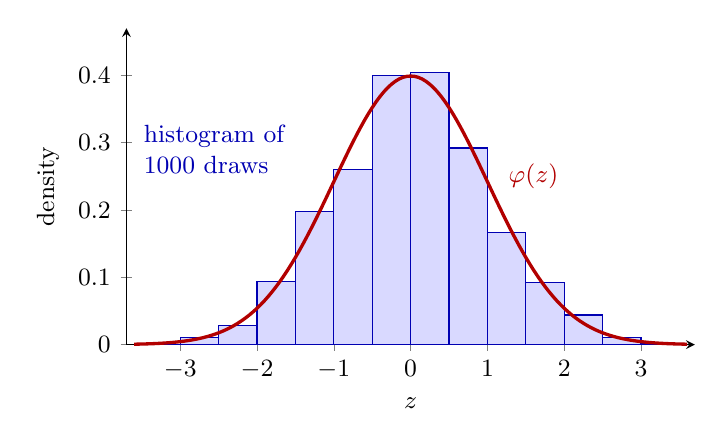
\begin{tikzpicture}[font=\small, >={Latex[length=2mm]}]
  \begin{axis}[width=8.8cm, height=5.6cm, axis lines=left, xmin=-3.7, xmax=3.7, ymin=0, ymax=0.47,
      xtick={-3,-2,-1,0,1,2,3}, ytick={0,0.1,0.2,0.3,0.4}, xlabel={$z$}, ylabel={density},
      tick label style={font=\small}, label style={font=\small}, clip=false]
    \addplot[ybar interval, fill=blue!15, draw=blue!70!black] coordinates {(-3.5,0) (-3,0.01) (-2.5,0.028) (-2,0.094) (-1.5,0.198) (-1,0.26) (-0.5,0.4) (0,0.404) (0.5,0.292) (1,0.166) (1.5,0.092) (2,0.044) (2.5,0.01) (3,0.002) (3.5,0.002)};
    \addplot[red!70!black, very thick, domain=-3.6:3.6, samples=145] {exp(-x^2/2)/sqrt(2*pi)};
    \node[red!70!black, anchor=west] at (axis cs:1.15,0.25) {$\varphi(z)$};
    \node[blue!70!black, anchor=west, align=left] at (axis cs:-3.6,0.29) {histogram of\\1000 draws};
  \end{axis}
\end{tikzpicture}
\end{document}
